\documentclass[nojss]{jss}\usepackage[]{graphicx}\usepackage[]{color}
%% maxwidth is the original width if it is less than linewidth
%% otherwise use linewidth (to make sure the graphics do not exceed the margin)
\makeatletter
\def\maxwidth{ %
  \ifdim\Gin@nat@width>\linewidth
    \linewidth
  \else
    \Gin@nat@width
  \fi
}
\makeatother

\definecolor{fgcolor}{rgb}{0.345, 0.345, 0.345}
\newcommand{\hlnum}[1]{\textcolor[rgb]{0.686,0.059,0.569}{#1}}%
\newcommand{\hlstr}[1]{\textcolor[rgb]{0.192,0.494,0.8}{#1}}%
\newcommand{\hlcom}[1]{\textcolor[rgb]{0.678,0.584,0.686}{\textit{#1}}}%
\newcommand{\hlopt}[1]{\textcolor[rgb]{0,0,0}{#1}}%
\newcommand{\hlstd}[1]{\textcolor[rgb]{0.345,0.345,0.345}{#1}}%
\newcommand{\hlkwa}[1]{\textcolor[rgb]{0.161,0.373,0.58}{\textbf{#1}}}%
\newcommand{\hlkwb}[1]{\textcolor[rgb]{0.69,0.353,0.396}{#1}}%
\newcommand{\hlkwc}[1]{\textcolor[rgb]{0.333,0.667,0.333}{#1}}%
\newcommand{\hlkwd}[1]{\textcolor[rgb]{0.737,0.353,0.396}{\textbf{#1}}}%

\usepackage{framed}
\makeatletter
\newenvironment{kframe}{%
 \def\at@end@of@kframe{}%
 \ifinner\ifhmode%
  \def\at@end@of@kframe{\end{minipage}}%
  \begin{minipage}{\columnwidth}%
 \fi\fi%
 \def\FrameCommand##1{\hskip\@totalleftmargin \hskip-\fboxsep
 \colorbox{shadecolor}{##1}\hskip-\fboxsep
     % There is no \\@totalrightmargin, so:
     \hskip-\linewidth \hskip-\@totalleftmargin \hskip\columnwidth}%
 \MakeFramed {\advance\hsize-\width
   \@totalleftmargin\z@ \linewidth\hsize
   \@setminipage}}%
 {\par\unskip\endMakeFramed%
 \at@end@of@kframe}
\makeatother

\definecolor{shadecolor}{rgb}{.97, .97, .97}
\definecolor{messagecolor}{rgb}{0, 0, 0}
\definecolor{warningcolor}{rgb}{1, 0, 1}
\definecolor{errorcolor}{rgb}{1, 0, 0}
\newenvironment{knitrout}{}{} % an empty environment to be redefined in TeX

\usepackage{alltt}

%%%%%%%%%%%%%%%%%%%%%%%%%%%%%%
%% declarations for jss.cls %%
%%%%%%%%%%%%%%%%%%%%%%%%%%%%%%
%\VignetteEngine{knitr::knitr}
%\VignetteIndexEntry{hviciPlotting}
%\VignetteIndexEntry{Generating plot.sas style figures in R}
%\VignetteKeywords{publication graphics, powerpoint, ggplot2, plot.sas}
%\VignetteDepends{ggplot2}
%\VignettePackage{hviciPlotting} 

%% almost as usual
\author{John Ehrlinger\\Cleveland Clinic} %\And \\Plus Affiliation}
\title{{\pkg{hviciPlotting}}: Generating \code{plot.sas} style figures in \proglang{R}}

%% for pretty printing and a nice hypersummary also set:
\Plainauthor{John Ehrlinger} %% comma-separated
\Plaintitle{hviciPlotting: Generating plot.sas style figures in R} %% without formatting
\Shorttitle{hviciPlotting: Generating plot.sas style figures}

%% an abstract and keywords
\Abstract{ 
We introduce the \proglang{R} package \pkg{hviciPlotting}, a set of tools for creating publication quality graphics in \proglang{R}. The \pkg{hviciPlotting} package is designed to replace the \code{plot.sas} macro we currently use in \proglang{SAS}. The package includes both \proglang{R} recipes for generating our standard graphics using \pkg{ggplot2} commands and a set of themes designed to format those figures for both manuscript and \code{PowerPoint} targets. 

The goal of this package vignette is to introduce the \pkg{hviciPlotting} methodology, as well as to document the best practices of creating our publication quality graphics for both manuscripts and power point presentations.

This document is included with the \pkg{hviciPlotting} package as a package vignette, installed into \proglang{R} when the package is installed, and view able using the \code{vignette("hviciPlotting")} command.
}
\Keywords{publication graphics, powerpoint, ggplot2, plot.sas}
\Plainkeywords{publication graphics, powerpoint, ggplot2, plot.sas}
%% at least one keyword must be supplied

%% publication information
%% NOTE: Typically, this can be left commented and will be filled out by the technical editor
%% \Volume{13}
%% \Issue{9}
%% \Month{September}
%% \Year{2004}
%% \Submitdate{2004-09-29}
%% \Acceptdate{2004-09-29}

%% The address of (at least) one author should be given
%% in the following format:
\Address{
  John Ehrlinger\\
  Quantitative Health Sciences\\
  Lerner Research Institute\\
  Cleveland Clinic\\
  9500 Euclid Ave\\
  Cleveland, Ohio 44195\\
%  Telephone: +41/0/44634-4643 \\
%  Fax: +41/0/44634-4386 \\
  E-mail: \email{john.ehrlinger@gmail.com}\\
  URL: \url{http://www.biostat.uzh.ch/aboutus/people/rufibach.html}
}

%% It is also possible to add a telephone and fax number
%% before the e-mail in the following format:
%% Telephone: +43/1/31336-5053
%% Fax: +43/1/31336-734

%% for those who use Sweave please include the following line (with % symbols):
%% need no \usepackage{Sweave.sty}

%% end of declarations %%%%%%%%%%%%%%%%%%%%%%%%%%%%%%%%%%%%%%%%%%%%%%%



\IfFileExists{upquote.sty}{\usepackage{upquote}}{}
\begin{document}

%% include your article here, just as usual
%% Note that you should use the \pkg{}, \proglang{} and \code{} commands.

\begin{knitrout}\footnotesize
\definecolor{shadecolor}{rgb}{0.969, 0.969, 0.969}\color{fgcolor}\begin{figure}[!htpb]


{\centering 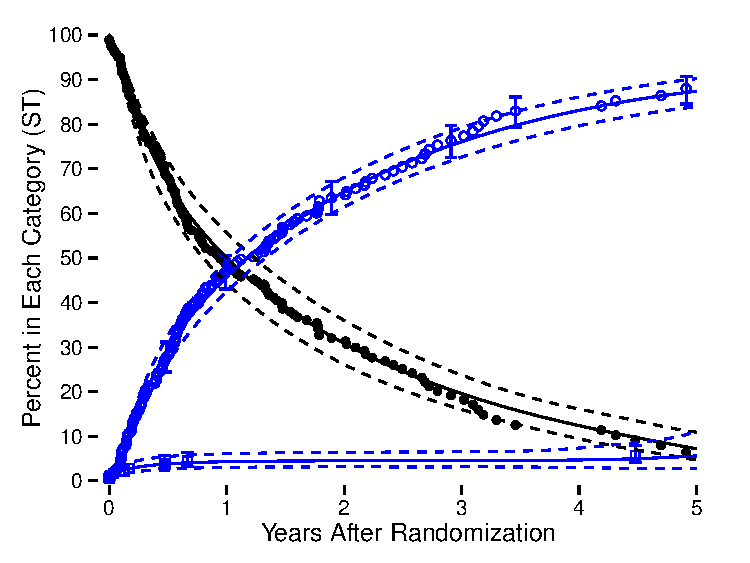
\includegraphics[width=\maxwidth]{figure/beamer-introFigure} 

}

\caption[Demonstration figure]{Demonstration figure\label{F:introFigure}}
\end{figure}


\end{knitrout}
% -----------------------------------------------------
\section{About this document}
% -----------------------------------------------------
This document is an introduction to the \proglang{R} package \pkg{hviciPlotting}, a set of tools for creating publication quality graphics in \proglang{R}. The package and this document describe the process of creating graphics in \proglang{R} that conform to the standards of the clinical investigations statistics group within The Heart \& Vascular Institute at the Cleveland Clinic. These graphics are analogous to those generated with the \code{plot.sas} macro in \proglang{SAS}.

This document is the package vignette for the \pkg{hviciPlotting} package, and as such is the primary documentation for the package. The latest version of the document can be obtained with the 
\begin{CodeChunk}
\begin{CodeInput}
R> vignette("hviciPlotting", package = "hviciplotting")
\end{CodeInput}
\end{CodeChunk}

The goal is to update this document as the package is updated to include all relevant changes for publication. 

% -----------------------------------------------------
\section{Introduction}
% -----------------------------------------------------
For many years, the mainstay for generating graphics for manuscripts and presentations in the statistics group in HVI has been the \code{plot.sas} macro using \proglang{SAS}. However, recently, we have had issues migrating this macro to newer versions of \proglang{SAS} ($> 8.0$) and MicroSoft Office products ($> 2003$). 

In an effort to alleviate the versifying problems, and to standardize the generation of figures within \proglang{R}, we have developed the \pkg{hviciPlotting} \proglang{R} package. The goal of the package, and this document, is simplify the creation of publication quality graphics in  \proglang{R}. We are specifically encoding the best practices of the HVI Clinical Investigations formatting, so that our statisticians will be able to simply create graphics for publication with a minimal amount of effort.

The \pkg{hviciPlotting} package also implements best practices for \proglang{R} graphics by leveraging the \pkg{ggplot2} package~\citep{Wickham:2009}. The \pkg{ggplot2} package is an implementation of the Grammar of Graphics~\citep{Wilkinson:2005}, which is a formalization of graphical concepts, and the building of graphical objects from a sequence of independent components. These components can be combined in many different ways.

The \code{plot.sas} macro is also an implementation of a graphics grammar. The grammar is derived from the ZETA pen plotters, which used GML (Graphics Machine Language) to control between 4 and and 8 colored pens for generating color line and point figures. Because both systems use a graphics language it is straight forward to translate commands between the two methods. 

This document outlines how to generate figures using the \pkg{ggplot2} and \pkg{hviciPlotting} packages. Our approach is to demonstrate the \proglang{R} commands to generate the same elements created with \code{plot.sas} commands. Section~\ref{S:plot.sas} gives an overview of the methodology of the \code{plot.sas} macro and Section~\ref{S:ggplot2tuple} details how to create line and point plots with \pkg{ggplot2}. A key part of \pkg{hviciPlotting} package is custom themes for figures. Once you have created your figure, Section~\ref{S:themes} details how to get the formatting correct for manuscripts or presentations. Section~\ref{S:saving} describes functions for saving the figures to simplify the import into publication documents.

% -----------------------------------------------------
\section[The plot.sas macro]{The \code{plot.sas} macro}\label{S:plot.sas}
% -----------------------------------------------------
To demonstrate the process, we first look at some example code using the \code{plot.sas} macro. This code is intended to generate a figure for manuscript publication and was modified to generate Figure~\ref{F:introFigure}. Note the first line of the code block indicates the location of the file.

\begin{CodeChunk}\small
\begin{CodeInput}
%let STUDY=/studies/cardiac/valves/aortic/replacement/
           partner_publication_office/partner1b/mortality_5y
*******************************************************************************;
* Bring in PostScript plot macro                                               ;
filename plt "!MACROS/plot.sas"; %inc plt;
filename gsasfile pipe 'lp';
*______________________________________________________________________________;
*                                                                              ;
*                       P O S T S C R I P T   P L O T S
*______________________________________________________________________________;
*                                                                              ;
* Multiple decrement, nonparametric and parametric                             ;
filename gsasfile "&STUDY/graphs/ce.states.ST_toJohn.both.ps";
%plot(goptions gsfmode=replace, device=pscolor, gaccess=gsasfile end;
id l="&STUDY/graphs/ce.states.ST_toJohn.sas percent", end;
labelx l="Years After Randomization", end;
axisx order=(0 to 5 by 1), minor=none, end;
labely l="Percent in Each Category (ST)", end;
axisy order=(0 to 100 by 10), minor=none, end;
\end{CodeInput}
\end{CodeChunk}

We interupt this command here for some explanation. The \code{plot.sas} macro call starts with the \code{\%plot} command. The first line sets global graphic values, including the file where the figure will be saved (see Section~\ref{S:saving}). Each \code{plot.sas} command is terminated with the \code{end;} statement. We'll look at each command type individually.

The \code{id l=} command sets the footnote text used for manuscript figures to identify where the figure is saved (see Section~\ref{S:saving}). The \code{labelx} and \code{labely} commands set the axis label text (Section~\ref{S:labels}) and the \code{axisx} and \code{axisy} set the scales for each axis locating text and tics (Section~\ref{S:scales}).

The \code{tuple} command builds up graphics objects within the figure plot window. The first set of tuple commands builds up a set of three elements containing both points (Section~\ref{S:points}) and errorbars (Section~\ref{S:errorbars}). Each \code{tuple} statement operates on a dataset indicated by the \code{set} command. 
\begin{CodeChunk}\small
\begin{CodeInput}
/******NON-PARAMETRIC: SYMBOLS AND CONFIDENCE BARS *******/
tuple set=green, symbol=dot, symbsize=1/2, linepe=0, linecl=0,
    ebarsize=3/4, ebar=1,
    x=iv_state, y=sginit, cll=stlinit, clu=stuinit, color=black, 
    end;
tuple set=green, symbol=circle, symbsize=1/2, linepe=0, linecl=0,
    ebarsize=3/4, ebar=1,
    x=iv_state, y=sgdead1, cll=stldead1, clu=studead1, color=blue, 
    end;
tuple set=green, symbol=square, symbsize=1/2, linepe=0, linecl=0,
    ebarsize=3/4, ebar=1,
    x=iv_state, y=sgstrk1, cll=stlstrk1, clu=stustrk1, color=blue, 
    end;
\end{CodeInput}
\end{CodeChunk}
Symbols shapes and sizes are specified with the \code{symbol} and \code{symbsize} commands (Section~\ref{S:shapes}).

The second set of \code{tuple} statements build up a set of three elements containing lines and confidence intervals (Section~\ref{S:lines}).
\begin{CodeChunk}\small
\begin{CodeInput}

/**********PARAMETRIC : SOLID LINES AND CONFIDENCE INTERVALS**********/      
tuple set=all, x=years, y=noinit, cll=clinit, clu=cuinit,
    width=0.5,color=black, 
    end;

tuple set=all, x=years, y=nodeath, cll=cldeath, clu=cudeath,
    width=0.5,color=blue, 
    end;

tuple set=all, x=years, y=nostrk, cll=clstrk, clu=custrk,
    linecl=2, width=0.5,color=blue, 
    end;
);
run;
*******************************************************************************;
\end{CodeInput}
\end{CodeChunk}

The \code{plot.sas} macro code is closed by the ending \code{);} characters, and \proglang{SAS} is instructed to \code{run;} the code. Running combines building the figure by combining elements from \code{label}, \code{axis} and \code{tuple} statements and saving it into the file specified by the \code{gsasfile} variable. Note that much of the figure formatting is mixed within the \code{tuple} statements using \code{width}, \code{color}, \code{linepe} and \code{linecl} commands. 


A similar set of \code{plot.sas} commands is used to create presentation graphics.

\begin{CodeChunk}\small
\begin{CodeInput}
*______________________________________________________________________________;
*                                                                              ;
*       C G M   F I L E S   F O R   P O W E R P O I N T   S L I D E S
*______________________________________________________________________________;
*                                                                              ;
* Competing risks, parametric only                                             ;
filename gsasfile "&STUDY/graphs/ce.states.ST_toJohn.cgm";
%plot(goptions gsfmode=replace, device=cgmmppa, ftext=hwcgm001, end;
axisx order=(0 to 5 by 1), minor=none, value=(height=2.4), end;
axisy order=(0 to 100 by 20), minor=none, value=(height=2.4), 
value=(height=2.4 j=r ' ' '20' '40' '60' '80' '100'), end;
tuple set=all, x=years, y=noinit, width=3, color=gray, end;
tuple set=all, x=years, y=nostrk, width=3, color=red, end;
tuple set=all, x=years, y=nodeath, width=3, color=blue, end;
);
run;  
\end{CodeInput}
\end{CodeChunk}
Differences include the target \code{device} and \code{ftext} as well as some handling of figure labels with \code{value} instead of \code{label} commands. We also have rules for what to and not to include in presentation graphics (Section~\ref{S:rules}).

% -----------------------------------------------------
\section[Generating ggplot2 graphics]{Generating \pkg{ggplot2} graphics}\label{S:ggplot2tuple}
% -----------------------------------------------------

\subsection{Lines}\label{S:lines}

\subsection{Points}\label{S:points}


\subsection{ErrorBars}\label{S:errorbars}

\subsection{Labels}\label{S:labels}

\subsection{Colors}\label{S:colors}


\subsection{Scales}\label{S:scales}

% -----------------------------------------------------
\section{Generating other figure types}\label{S:alternateFigures}
% -----------------------------------------------------

\subsection{Bar Charts}

\subsection{Histograms}

\subsection{Additional Figure Types}


% -----------------------------------------------------
\section[Themes for publications]{\pkg{ggplot2} themes for publication}\label{S:themes}
% -----------------------------------------------------

\subsection{Theme for Manuscripts}

\subsection{Theme for Presentations}

% -----------------------------------------------------
\section{Saving Publication graphics}\label{S:saving}
% -----------------------------------------------------

\subsection{Manuscript graphics}

\subsection{PowerPoint graphics}

% -----------------------------------------------------
\section{Graphics rules to live by}\label{S:rules}
% -----------------------------------------------------

% =======================================
\section{Conclusions} \label{S:concl}
% =======================================
In this article, we present some functions in the \pkg{hviciPlotting} package for \proglang{R} 

% =======================================
% \section{Literatur} \label{sec: references}
% =======================================
%\nocite{*}

\bibliography{hviciPlotting}



\end{document}
